\documentclass[11pt, a4paper]{article}

% ── 编码与中文支持 ──
\usepackage[UTF8]{ctex}
\usepackage{fontspec}
\setmainfont{Times New Roman}
\setCJKmainfont{SimSun}[BoldFont=SimHei, ItalicFont=KaiTi]

% ── 页面与排版 ──
\usepackage[margin=2.54cm]{geometry}
\usepackage{setspace}
\onehalfspacing
\usepackage{ragged2e}
\justifying

% ── 参考文献 APA 7 ──
\usepackage[style=apa, backend=biber, natbib=true]{biblatex}
\addbibresource{references.bib}

% ── 图表 ──
\usepackage{graphicx}
\usepackage{booktabs}
\usepackage{tabularx}
\usepackage{float}
\graphicspath{{figures/}}

% ── 其他 ──
\usepackage{hyperref}
\hypersetup{colorlinks=true, linkcolor=blue, citecolor=blue, urlcolor=blue}
\usepackage{caption}
\usepackage{subcaption}
\usepackage{enumitem}
\usepackage{longtable}

% ── 标题信息 ──
\title{
  亚洲女大学生校园健身房空间、身体意象与阻力训练回避研究\\[0.5em]
  \normalsize Spatial Environment, Body Image, and Resistance Training Avoidance\\
  among Asian Female College Students in Campus Gyms
}
\author{
  {\small Bo Yu, Xingjian Li, Yiran Dong, Xiangnan Gao, Jianzhuo Yuan, Yunfan Lu}
}
\date{
  \small UCUG 1808 --- Sport in Society, 25/26 Spring Semester\\
  \small Final Group Research Project
}

\begin{document}

\maketitle
\thispagestyle{empty}

\begin{abstract}
本研究采用混合方法设计，结合在线问卷（$N = 32$）与半结构化访谈（$n = 3$），考察亚洲女大学生在校园健身房中对阻力训练的回避机制。
结果显示，78.13\% 的参与者使用过学校健身房，但仅 15.63\% 最常使用自由重量区。
空间压迫/训练焦虑与回避频率呈较强正相关（Spearman's $\rho = .65$, $p < .001$），而社交媒体审美内化与回避的相关较弱且未达到显著水平（$\rho = .31$, $p = .084$）。
``不想练出明显肌肉''作为回避原因为 0\%，表明回避主要不是由对肌肉化的恐惧驱动，而是来自空间可见性、新手门槛和器械知识不足的叠加压力。
受访者普遍采用错峰、同伴陪伴等策略性协商方式进入健身房，而非完全退出运动。
96.88\% 的参与者支持学校提供女性初学者力量训练 workshop。
研究建议高校通过入门指导、半私密分区和叙事转变降低自由重量区的进入成本，使性别平等从形式上的设备开放走向实际的空间可达。

\noindent\textbf{Keywords: } resistance training avoidance, gym intimidation, spatial pressure, body image, female college students, mixed methods
\end{abstract}

\newpage

% ── 目录（提交时可删除）──
\tableofcontents
\newpage

% ── 正文各节 ──
\section{Introduction}

University campus gyms are commonly imagined as open health spaces accessible to all students, yet their actual accessibility is far from equal.
In free-weight and strength training areas in particular, female students enter less frequently, stay for shorter durations, and exhibit more pronounced avoidance.
A recent survey of 357 female college students found that respondents reported moderate levels of gym intimidation on the \textcite{levinson2013seam} subscale, and that this intimidation had become a significant barrier to exercise participation; the same study also noted higher avoidance among lower-year students \parencite{rendall2024gym}.
Consistent with this finding, qualitative research on female gym users has shown that the intense gender segregation, masculine performance, sense of being watched, and spatial atmosphere of ``always being on display'' in the weight area can transform what should be a public training environment into a threshold that requires considerable courage to cross \parencite{turnock2021gyms}.

If campus gyms impose a form of physical spatial pressure, image-based social media platforms continuously generate a digital form of body pressure.
Existing research indicates that the link between social media and body image concerns does not operate primarily through ``screen time'' per se, but rather indirectly through appearance ideal internalization, appearance comparison, and appearance-related self-presentation \parencite{fardouly2016social}.
Research on young women further demonstrates that the relationship between social media use intensity and negative body image is mediated through the ``ideal internalization--social comparison'' chain \parencite{jung2022social}; experimental studies have also found that even fitspiration images, which ostensibly promote ``health and discipline,'' can immediately elevate body dissatisfaction and negative mood \parencite{tiggemann2015fitspiration}.

For the present study, what is more critical is that these two forms of pressure are not independent of each other.
Research on Chinese female college students has shown that media and peers influence negative body image through appearance comparison and thin-ideal internalization \parencite{shen2022media}; in a sample of young Chinese women, selfie posting and body comparison on social networks were significantly associated with body surveillance, weight-control exercise, and restrictive eating \parencite{yao2020selfie}.
In other words, many women are not simply ``unwilling to exercise''; rather, they are simultaneously navigating two sets of pressures:
on one hand, the free-weight area appears to be someone else's territory; on the other hand, digital media constantly reminds them that a woman's body should ideally remain slender and aesthetically pleasing, with some women also expressing concerns about appearing ``too muscular'' from strength training \parencite{peters2019barriers}.
Narrative research on Chinese women's fitness experiences also reminds us that fitness can be both a practice of agency and, simultaneously, a form of bodily discipline shaped by aesthetic norms \parencite{xiong2021fanshen}.

Building on this foundation, the present study focuses on resistance training participation among female college students in Chinese universities, attempting to answer a question with broader sociological significance:
When physical exercise spaces are experienced as male-dominated, and digital aesthetic standards continuously reinforce the norms of a ``correct female body,'' how do women understand, choose, and avoid certain forms of training?
The overarching goal of this study is to examine how the spatial environment of campus gyms and social media appearance norms jointly shape female college students' attitudes, preferences, and participation behaviors regarding resistance training.
Although the sample is drawn from a single Chinese university, the theoretical framework is intended to have broader relevance to Asian campus contexts where similar gendered spatial dynamics and digital beauty norms operate.
Around this goal, this paper poses three research questions:

\begin{enumerate}[label=RQ\arabic*:, leftmargin=*]
  \item How do the spatial environment of campus gyms and gym intimidation influence female college students' resistance training avoidance?
  \item To what extent does the internalization of social media appearance norms shape female students' exercise preferences?
  \item How do female students negotiate between ``exercising for health'' and ``fear of deviating from digital appearance norms''?
\end{enumerate}

This study carries dual significance.
Theoretically, it does not simply explain women's avoidance of campus gyms as a lack of personal motivation; instead, it places space, gaze, comparison, appearance internalization, and training choices within a single analytical framework, thereby addressing the fragmentation in existing research that examines ``body image only'' or ``exercise participation only.''
Practically, this issue directly concerns whether the allocation of campus physical education resources has genuinely achieved equitable accessibility:
if female students nominally have access to the gym but are effectively excluded from the free-weight area by spatial layout, body anxiety, and appearance concerns, then ``campus health promotion'' remains incomplete.

The structure of this paper is as follows: the next section reviews the relevant literature on gendered gym spaces, resistance training barriers, body objectification, and social media appearance norms; the subsequent section describes the methods and data limitations of this study; the results section presents the questionnaire aggregate data and interview themes; the discussion section is organized around four themes---spatial pressure, beginner barrier, appearance influence, and strategic negotiation---with responses to the three research questions embedded within each subsection.

\section{Literature Review, Research Gaps, and Theoretical Framework}

\subsection{Gendered Space in Campus Gyms}

Campus gyms are not neutral containers but spatial practices continuously shaped by social relations.
Research on women's entry into gyms has repeatedly shown that the weight area is not merely delineated by equipment---it is simultaneously encoded with gendered meanings:
the concentration of equipment, the high intensity of movements, the prominent noise, the extended equipment occupancy times, and the greater visibility of male users all contribute to its being experienced as a ``male space.''
\textcite{turnock2021gyms}'s qualitative study of commercial gyms makes this point especially clear:
women's barriers to entry arise not only from whether ``women know how to train,'' but from the sharp gendered segregation of the weight area, the emotional threshold of crossing into that space, the performance of masculinity within it, and the discomfort of being continuously exposed to others' gazes.
\textcite{rendall2024gym}'s recent study of female college students further demonstrates that this spatial deterrence is not an isolated narrative but a measurable, significant phenomenon within their campus female sample.
These findings establish that gendered spatial encoding is a precondition for understanding why women's training participation takes specific avoidance forms---a question to which the resistance training literature now turns.

\subsection{Barriers to Resistance Training}

Alongside spatial barriers are participation barriers specific to resistance training itself.
\textcite{peters2019barriers} surveyed college-aged women and identified resistance training barriers as a distinct phenomenon rather than a subcomponent of general physical inactivity: women reported lack of knowledge about proper technique, uncertainty about how to design a training program, perceived social judgment in the weight room, and limited access to guidance or instruction.
These barriers are compounded by the gendered spatial dynamics discussed above: when the free-weight area is already experienced as a ``male space,'' the absence of equipment knowledge and instructional support makes entry even more daunting.
\textcite{rendall2024gym}'s finding that gym intimidation---measured through the SEAM subscale \parencite{levinson2013seam}---functions as a significant exercise barrier among female college students further supports the view that spatial and knowledge-based barriers are intertwined rather than independent.
For this reason, the present study treats ``resistance training avoidance'' rather than ``insufficient physical activity'' as the more precise behavioral outcome variable, asking why a considerable proportion of women concentrate their exercise practices on cardio and light toning while avoiding free weights.
These participation barriers, however, do not arise in a vacuum; they are experienced through gendered bodies already shaped by processes of objectification and surveillance.

\subsection{Objectification and Body Surveillance}

If spatial theory helps us understand ``where entry becomes difficult,'' theories of the female body help us understand ``why the same space is more hostile to certain bodies.''
This study maintains its theoretical anchoring in \textcite{lefebvre1991production} and \textcite{beauvoir1949second}:
the former helps us understand that space is not a neutral given but a product of power relations; the latter frames the female body as an experiential process of being shaped, evaluated, and objectified under the social gaze.
At the level of empirical operationalization, this line of inquiry aligns closely with \textcite{fredrickson1997objectification}'s objectification theory.
This theory posits that women's tendency to treat their own bodies as objects to be scrutinized is not merely an individual psychological deficit but is tied to enduring sociocultural structures of gendered looking.
In gym environments---characterized by abundant mirrors, open sight lines, movements that can easily be performed ``incorrectly,'' and the high visibility of others' bodily displays---this body surveillance becomes more likely to translate into shame, anxiety, and avoidance.
Crucially, the body surveillance triggered in gym spaces does not operate in isolation; it is amplified by an increasingly pervasive digital culture of appearance norms, which the next section examines.

\subsection{Social Media Beauty Norms and Internalization}

Social media appearance norms provide a continuous cultural backdrop for this spatial anxiety.
Relevant reviews and systematic reviews have converged on the finding that social network use is consistently associated with body image disturbance, disordered eating outcomes, and appearance-based self-surveillance, with appearance comparison and appearance ideal internalization serving as key mechanisms \parencite{holland2016systematic}.
\textcite{jung2022social}'s study of young women further indicates that the effect of social media use intensity on body image is primarily mediated by appearance ideal internalization and social comparison, rather than being a simple time-exposure effect.
For young women today, what warrants attention is no longer merely the traditional thin ideal, but the fit ideal that simultaneously emphasizes ``slimness,'' ``firmness,'' ``self-discipline,'' and ``health as display.''
\textcite{donovan2020fitideal} thus argue that ``strong is the new skinny'' does not mean the disappearance of appearance pressure; rather, the pressure has shifted from ``must be thin'' to ``must be strong in the right way.''
This finding is highly consistent with \textcite{tiggemann2015fitspiration}'s experimental evidence:
fitspiration images that appear positively motivated may nonetheless undermine women's body satisfaction in a short period of time.
These findings, however, are predominantly situated within Western media ecosystems; whether and how they manifest in East Asian digital cultures---where beauty norms, fitness discourses, and body ideals may follow different logics---requires further contextualization.

\subsection{The East Asian and Chinese Context}

Placing this research chain within the East Asian and Chinese context renders the issues even more concrete.
Chinese college student research has shown that media and peers influence negative body image through appearance comparison and thin ideal internalization \parencite{shen2022media}, and that Chinese young women's social media practices are linked to body surveillance, weight-control exercise, and restrictive eating:
\textcite{yao2020selfie} found that selfie posting and body surveillance promote a tendency toward ``exercising to control weight'';
another study of Chinese female college students showed that SNS body comparison can influence restrictive eating through body shame \parencite{yao2021bodyimage}.
In other words, in Chinese samples, social media does not merely ``make people unhappy''---it may also shape how people understand exercise, why they exercise, and whether they pursue bodily capability or appearance management.
However, this process should not be understood as one-dimensional passive compliance.
Through the fitness narratives of 12 Chinese women, \textcite{xiong2021fanshen} situates dieting, weight loss, body management, fitness sociality, body stereotypes, self-identity, and cultural aesthetics within a single experiential landscape, suggesting that women's fitness may be organized by appearance norms but may also become part of life planning, self-understanding, and bodily capability reconstruction.
Thus, women may oscillate among discipline, sociality, self-formation, emotional recovery, and agentic negotiation.
This agentic dimension is important because it suggests that women are not simply passive recipients of spatial and appearance pressures---yet whether and how such agency operates specifically within campus gym free-weight areas remains underexplored.

\subsection{Research Gaps}

The existing literature has thus separately addressed gendered space in gyms, social media body image, and appearance pressure among Chinese college students, yet a clear intersectional gap remains:
First, research on women's gym entry barriers has predominantly focused on European and American commercial gyms or general female samples, with limited direct attention to the more specific context of ``Asian female college students + campus gyms + free-weight area.''
Second, research on Chinese college students' body image and social media has primarily focused on negative body image, body shame, restrictive eating, and selfie behavior, with less attention to connecting these psychological and cultural mechanisms to specific training choices within campus fitness spaces.
Third, spatial pressure and digital appearance pressure have typically been studied separately rather than examined simultaneously within a mixed methods framework.
The value of the present study lies precisely in bringing these two usually separate questions together.

\subsection{Integrated Theoretical Framework}

Drawing on the above literature, this study proposes an integrated theoretical framework.
The first layer is \textbf{spatial production logic}: as demonstrated by \textcite{turnock2021gyms} and \textcite{rendall2024gym}, the free-weight area in campus gyms is not a naturally formed training venue but is continuously constructed as a male-dominated area through its layout, equipment, user composition, social norms, and bodily display; this spatial encoding translates into contextualized social exercise anxiety and gym avoidance.
The second layer is \textbf{body objectification and appearance internalization logic}: following \textcite{fredrickson1997objectification} and extending the media effects literature reviewed above \parencite{holland2016systematic,jung2022social}, women are more likely to engage in body surveillance in image-based media and public exercise environments, transforming external appearance standards into self-imposed requirements.
The third layer is the \textbf{behavioral outcome layer}: as suggested by \textcite{peters2019barriers}'s identification of resistance training as a distinct behavioral domain and \textcite{xiong2021fanshen}'s account of agentic negotiation in women's fitness, when ``this space does not belong to me'' and ``my body must not deviate from the ideal femininity'' co-occur, women are more likely to concentrate their exercise choices on cardio, fat loss, light toning, or peripheral machine areas, while exhibiting avoidance, postponement, strategic negotiation, or conditional entry with respect to free-weight training.

This integrated framework also naturally corresponds to the present study's measurement design:
SEAM is suited to capturing contextualized social exercise anxiety and avoidance; SATAQ-4 provides a measurement reference for understanding media pressure and appearance ideal internalization; and semi-structured interviews are used to complement the narrative dimension of ``how they explain, experience, and negotiate these pressures.''

\section{Methodology}

\subsection{Research Design}

This study adopts a small-sample mixed methods design, combining descriptive results from an online questionnaire with semi-structured interview materials to examine how Asian female college students understand the relationship among campus gym space, body image pressure, and resistance training avoidance.
A mixed-methods design was chosen because the research questions require both an overview of group-level patterns and an in-depth understanding of individual experience mechanisms.
Questionnaire data can reveal which spatial perceptions and avoidance reasons are most prominent, but the aggregate export format limits individual-level inference; conversely, interviews can capture contextual nuance, yet a sample of three cannot estimate population tendencies.
By integrating both, the study addresses the gap identified in the literature review, where spatial pressure and digital appearance pressure have typically been examined separately rather than within a single analytical framework.
The original design followed a sequential explanatory mixed methods approach: the questionnaire would first establish overall trends, followed by qualitative interviews to explain those trends.
After actual data collection, the quantitative component comprised item-level aggregate export tables from the survey platform and a subsequently supplemented participant-level response matrix; the qualitative component consisted of one-on-one semi-structured interview transcripts from 3 interviewees.
Therefore, beyond descriptive statistics, this study supplements the analysis with small-sample exploratory individual-level reliability, correlation, and group comparisons, but does not conduct multivariate regression, mediation modeling, or causal inference.

This adjustment does not alter the research questions themselves, but rather the strength and mode of expression of the evidence.
Quantitative results are used to illustrate which spatial perceptions, avoidance reasons, and intervention preferences are more prominent in the sample and to preliminarily examine bivariate relationships among spatial pressure, media appearance internalization, and free-weight area avoidance; qualitative materials are used to explain the contextual mechanisms behind these numbers.
This study continues to use SEAM's approach to measuring social exercise anxiety and avoidance \parencite{levinson2013seam}, SATAQ-4's approach to measuring sociocultural appearance internalization \parencite{schaefer2015sataq4}, and research on gendered gym space \parencite{turnock2021gyms,rendall2024gym} as theoretical references, but does not claim to have used the complete original scales.

\subsection{Participants and Data Sources}

The questionnaire was distributed online via the Wenjuanxing platform, with links shared to WeChat groups and Moments of the HKUST-GZ Class of 2024, recruiting participants through convenience sampling.
Data collection took place from April 30 to May 4, 2026.
A total of 34 individuals initiated the questionnaire.
Inclusion criteria were: (a) current university student status (Question 1, 33 passed); (b) self-identified as female (Question 2, 32 passed).
The core analytical sample was therefore $N = 32$ female university students.
The age distribution was concentrated in the 18--20 range (87.50\%), with 3 individuals aged 21--23 (9.38\%) and 1 individual aged 24 and above (3.13\%).
Because the questionnaire did not separately measure ethnicity, nationality, or ethnic identity, ``Asian female college students'' in this paper primarily refers to female students enrolled at the university within the Chinese-language and Asian campus context of this study; the findings should not be generalized as the universal experience of all Asian female students.

Qualitative materials were drawn from semi-structured interviews with 3 interviewees; interview topics were consistent with the questionnaire, focusing on campus gym experiences, perceptions of the free-weight area, experiences of being watched or evaluated, social media appearance content, exercise goals, and suggestions for university support measures.
The 3 interviewees had varied experiences: one used the gym and strength training area more frequently, one had begun strength training that semester due to coursework, and one trained primarily in the dormitory and had only briefly entered the gym.
This variation facilitated comparison of how ``relatively familiar users,'' ``recent entrants,'' and ``marginal/avoiders'' differently understood the same space.

\subsection{Survey Instrument}

The questionnaire comprised 29 items.
Items 1--2 were screening questions; Items 3--9 collected age, exercise frequency, campus gym use, commonly used areas, strength training experience, and exercise goals.
Items 10--15 used 1--5 slider scales to measure spatial pressure and training anxiety in the free-weight area, including difficulty accessing the layout, discomfort when more men are present, feelings of evaluation from mirrors and public visibility, concern about incorrect form, perceptions of a male-dominated atmosphere, and reluctance to stay due to crowding and equipment concentration.
Items 16--18 measured the frequency of active avoidance of the free-weight area, reasons for avoidance, and coping strategies.
Items 19--23 measured social media use and the influence of appearance content, with Items 21--23 using 1--5 slider scales.
Item 24 measured training self-efficacy for exercise goals; Items 25--27 measured acceptance of three types of potential interventions: reducing stereotypes, increasing semi-private partitioning or visual screening, and offering beginner-friendly women's strength training workshops.

Compared with the originally planned 60--100 individual-level questionnaires and 5--6 person qualitative group interviews from the proposal, the final available sample size was smaller.
However, the subsequently supplemented text-based Excel file provided each participant's item-level responses from Item 3 onward, so this study reports both the valid sample size per item, option frequencies, slider item means, score range proportions, and individual-level construct means.
Sliders were exported by the survey platform into five segments: 1--1.8, 1.9--2.6, 2.7--3.4, 3.5--4.2, 4.3--5.
This paper merges the two upper segments (3.5--5) as the ``upper score range'' to describe the proportion of respondents who strongly endorsed a given judgment.
Individual-level construct scores were calculated as the mean of relevant items: Items 10--15 for spatial pressure/training anxiety, Items 21--23 for social media appearance internalization, Item 24 as a single-item measure of training self-efficacy, and Items 25--27 for the intervention preference index.
Because Items 25--27 each target different intervention modalities, this paper treats them as a preference item set rather than a strict reflective psychological scale.

\subsection{Qualitative Procedure and Analysis}

All 3 interviews were conducted face-to-face offline, each lasting approximately 20 minutes; interviews were audio-recorded throughout, automatically transcribed using OpenAI Whisper, and the researcher subsequently proofread and anonymized the transcripts.
Interviews followed a semi-structured protocol but allowed interviewees to elaborate based on personal experience.
Questions entered through specific scenarios, such as the feeling of first entering the gym, differences between the cardio area and the strength area, concerns about form being evaluated, whether social media influenced exercise choices, and what kind of courses or spatial support they wished the university would provide.
Interview materials were organized into a Q\&A format and anonymized; during analysis, interviewees are referred to only as P1, P2, and P3.

Qualitative analysis followed a thematic analysis approach.
The first step involved repeated reading of the 3 transcripts, marking meaning units relevant to the research questions; the second step involved initial coding around spatial visibility, beginner barrier, male-dominated atmosphere, strategic negotiation, appearance influence, and intervention needs; the third step involved merging related codes into themes and using representative quotes to test whether the themes could explain the quantitative findings.
Because the sample consisted of only 3 interviewees, the thematic analysis did not aim for saturation or broad generalization, but rather served to explain the higher levels of spatial pressure, avoidance, and intervention preferences observed in the questionnaire.

To enhance the trustworthiness of the qualitative analysis, the researcher proofread each Whisper-generated transcript against the original audio for accuracy.
The three-step thematic procedure involved iterative reading, coding, and revision rather than a single pass.
The research team included members who share the demographic background of the study population (Chinese female university students with campus gym experience), which facilitated cultural understanding of interview narratives but also required conscious reflexivity about potential confirmation bias.
Due to the time constraints of the course project, member checking was not conducted; this limitation is acknowledged.

\subsection{Data Analysis}

Quantitative data were organized and summarized using Python.
The analysis script first parsed the aggregate Excel table exported by the survey platform, breaking down items, option frequencies, slider means, and segment frequencies into structured tables; it then read the participant-level response matrix to generate a de-identified participant score table.
At the individual level, this paper calculated Cronbach's $\alpha$ for spatial pressure/training anxiety and social media appearance internalization, used Spearman's $\rho$ to test exploratory correlations between construct scores and free-weight area avoidance frequency, and used Mann--Whitney $U$ tests to compare differences between frequent and infrequent free-weight area users and between those with and without systematic strength training experience.
All $p$ values are interpreted as small-sample exploratory evidence and are not used for strong causal claims.
Qualitative data were similarly processed using Python to parse Markdown interview texts, generating Q\&A tables, thematic coding tables, and representative quote tables.

Integration of quantitative and qualitative data occurred in the results and discussion sections.
This paper first reports high-frequency phenomena from the questionnaire, then uses interviews to explain how these phenomena are experienced by interviewees as mirror visibility, male numerical dominance, fear of incorrect form, equipment knowledge barriers, and strategic entry.
This integration approach suits the current data format: bivariate statistics can indicate whether variables co-vary but cannot establish statistical causation; interview materials help form a contextualized evidence chain regarding gendered entry barriers in campus gyms.

\subsection{Ethical Considerations}

This study discusses body image, feelings of being watched, and gym discomfort, which may touch upon shame, anxiety, or self-evaluation pressure.
Both the questionnaire and interviews were based on the principles of voluntary participation, anonymous processing, and the right to withdraw at any time; participants were informed of the study's purpose before responding, and interview recordings were conducted with the interviewees' informed consent.
Interview materials are presented in this report using only de-identified quotes (P1, P2, P3), avoiding the disclosure of details that could identify individuals.
This project is a course research project and has not been reviewed by a formal institutional ethics review committee, but the research process followed the ethical guidelines for coursework; the results are used solely for course paper writing and are not intended for individual diagnosis or institutional administrative evaluation.

\section{Results}

In the following results, item means, option frequencies, and upper score range proportions are derived from the questionnaire platform's aggregate export table; internal consistency coefficients, exploratory correlations, and group comparisons are based on the subsequently compiled participant-level response matrix ($N = 32$).

\subsection{Sample Characteristics}

The core questionnaire sample consisted of 32 female college students.
The majority were aged 18--20 (28 participants, 87.50\%).
Regarding exercise frequency in the past month, 15 participants (46.88\%) exercised 2--3 times per week, 6 (18.75\%) exercised once per week, 6 (18.75\%) exercised 4 or more times per week, and 5 (15.63\%) rarely exercised.
Twenty-five participants (78.13\%) had used the campus gym, while 7 (21.88\%) had not.

Gym area usage showed marked differences.
The most frequently selected area was the cardio area with treadmills, ellipticals, and similar equipment (21 participants, 65.63\%), followed by the fixed machine area (9 participants, 28.13\%).
Only 5 participants (15.63\%) selected the free-weight area, and 8 participants (25.00\%) reported that they generally did not enter the gym.
Strength training experience was also limited: 10 participants (31.25\%) had no exposure at all, 14 (43.75\%) had tried it but not systematically, and only 5 (15.63\%) were currently engaged in regular strength training.
Regarding exercise goals, fat loss/slimming was the most common (18 participants, 56.25\%), followed by toning/sculpting and improving fitness at 11 participants each (34.38\%), and building strength at 6 participants (18.75\%).

\begin{table}[H]
\centering
\caption{Sample Exercise Experience and Gym Usage Overview ($N = 32$)}
\label{tab:sample_actual}
\begin{tabular}{lll}
\toprule
Variable & Main Result & Percentage \\
\midrule
Has used campus gym & 25 participants & 78.13\% \\
Exercises 2--3 times per week & 15 participants & 46.88\% \\
Most frequently uses cardio area & 21 participants & 65.63\% \\
Most frequently uses free-weight area & 5 participants & 15.63\% \\
No strength training experience at all & 10 participants & 31.25\% \\
Some unsystematic attempts & 14 participants & 43.75\% \\
Currently engaged in regular strength training & 5 participants & 15.63\% \\
Primary goal is fat loss/slimming & 18 participants & 56.25\% \\
Primary goal is building strength & 6 participants & 18.75\% \\
\bottomrule
\end{tabular}
\end{table}

Figure \ref{fig:gym_area_use} more intuitively shows that the free-weight area accounts for a markedly lower proportion of commonly used areas compared to the cardio area.

\begin{figure}[H]
\centering
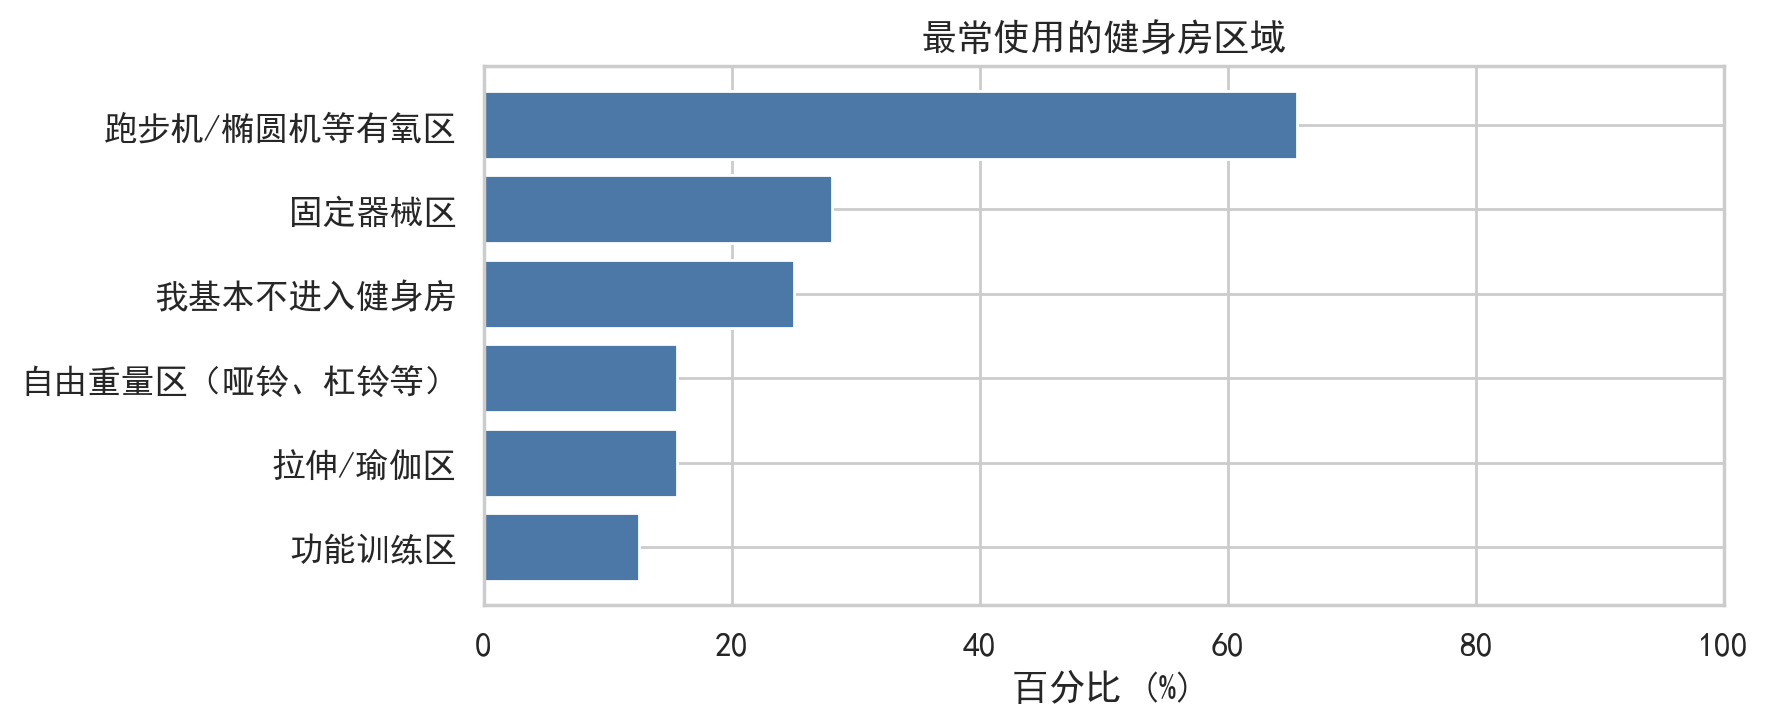
\includegraphics[width=0.85\textwidth]{gym_area_use.png}
\caption{Most Frequently Used Gym Areas}
\label{fig:gym_area_use}
\end{figure}

\subsection{Spatial Pressure and Free-Weight Avoidance}

The spatial pressure/training anxiety construct comprised Items 10--15, with an individual-level mean of 3.72 ($SD = 0.77$) and good internal consistency (Cronbach's $\alpha = .81$).
The most prominent item was ``I feel noticeably uncomfortable when there are many men in the free-weight area'' ($M = 4.24$, upper score range 81.25\%), followed by ``The population density, equipment concentration, and crowding in the free-weight area make me not want to stay'' ($M = 3.88$, upper score range 75.00\%) and ``I worry that if my form is incorrect, I will be noticed or judged by others'' ($M = 3.81$, upper score range 65.63\%).
This indicates that participants' discomfort does not stem solely from abstract body anxiety, but is concentrated in specific spatial conditions such as male predominance, open visibility, form errors, and crowded conditions that discourage lingering.

\begin{table}[H]
\centering
\small
\caption{Spatial Pressure/Training Anxiety Item Summary}
\label{tab:spatial_items_actual}
\begin{tabularx}{\textwidth}{lXcc}
\toprule
Item & Brief Description & Mean & Upper Score Range \\
\midrule
Q10 & Overall layout of the free-weight area feels inaccessible & 3.19 & 40.63\% \\
Q11 & Noticeably uncomfortable when many men are present & 4.24 & 81.25\% \\
Q12 & Mirrors and openly visible environment heighten sense of being evaluated & 3.57 & 53.13\% \\
Q13 & Worry about being noticed or judged for incorrect form & 3.81 & 65.63\% \\
Q14 & Free-weight area feels more like a male-dominated space & 3.61 & 62.50\% \\
Q15 & Population density, equipment concentration, and crowding reduce willingness to stay & 3.88 & 75.00\% \\
\bottomrule
\end{tabularx}
\end{table}

The participant-level data further support this interpretation.
After coding responses from ``never'' to ``always'' as 1--5, the mean frequency of actively avoiding the free-weight area was 3.09 ($SD = 1.33$).
Spatial pressure/training anxiety was moderately to strongly positively correlated with free-weight area avoidance frequency (Spearman's $\rho = .65$, $p < .001$).
Spatial pressure was also positively correlated with the intervention preference index ($\rho = .67$, $p < .001$), indicating that participants who felt greater spatial pressure in the free-weight area were more inclined to support measures such as workshops, semi-private partitioning, and stereotype reduction.

\begin{table}[H]
\centering
\small
\caption{Individual-Level Construct Descriptives and Reliability ($N = 32$)}
\label{tab:participant_scales}
\begin{tabular}{lcccc}
\toprule
Construct/Item Set & No. of Items & Mean & $SD$ & Cronbach's $\alpha$ \\
\midrule
Spatial pressure/training anxiety & 6 & 3.72 & 0.77 & .81 \\
Social media appearance internalization & 3 & 2.66 & 0.93 & .76 \\
Training self-efficacy & 1 & 3.49 & 0.94 & -- \\
Intervention preference index & 3 & 3.98 & 0.54 & N/A \\
\bottomrule
\end{tabular}
\end{table}

\begin{table}[H]
\centering
\small
\caption{Key Exploratory Spearman Correlations}
\label{tab:spearman_results}
\begin{tabular}{lcc}
\toprule
Variable Pair & $\rho$ & $p$ \\
\midrule
Spatial pressure/training anxiety -- Free-weight area avoidance frequency & .65 & $< .001$ \\
Spatial pressure/training anxiety -- Intervention preference index & .67 & $< .001$ \\
Intervention preference index -- Free-weight area avoidance frequency & .45 & .009 \\
Social media appearance internalization -- Free-weight area avoidance frequency & .31 & .084 \\
Training self-efficacy -- Free-weight area avoidance frequency & -.11 & .562 \\
\bottomrule
\end{tabular}
\end{table}

Figure \ref{fig:spatial_anxiety} shows the score distribution for each item of the spatial pressure/training anxiety construct.
The upper score range was most concentrated for items regarding male predominance, crowded conditions, and fear of incorrect form.

\begin{figure}[H]
\centering
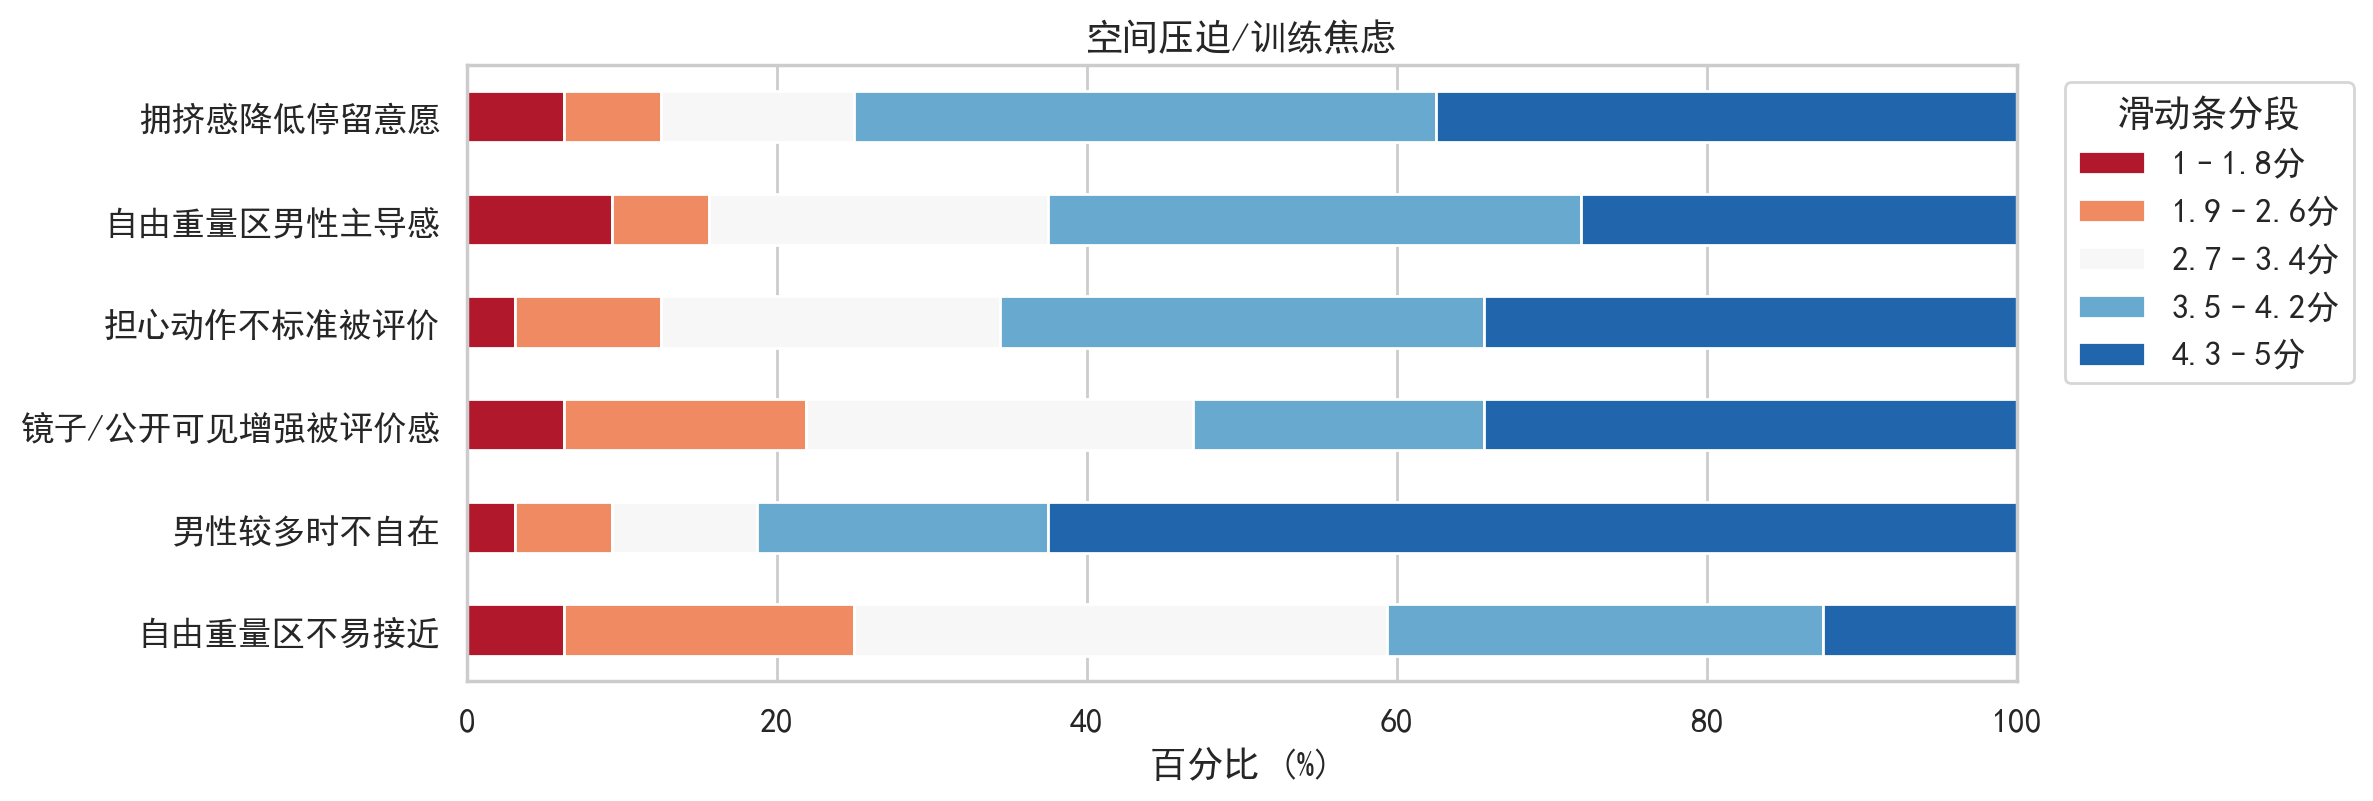
\includegraphics[width=\textwidth]{slider_spatial_anxiety.png}
\caption{Spatial Pressure/Training Anxiety Slider Distribution}
\label{fig:spatial_anxiety}
\end{figure}

\begin{figure}[H]
\centering
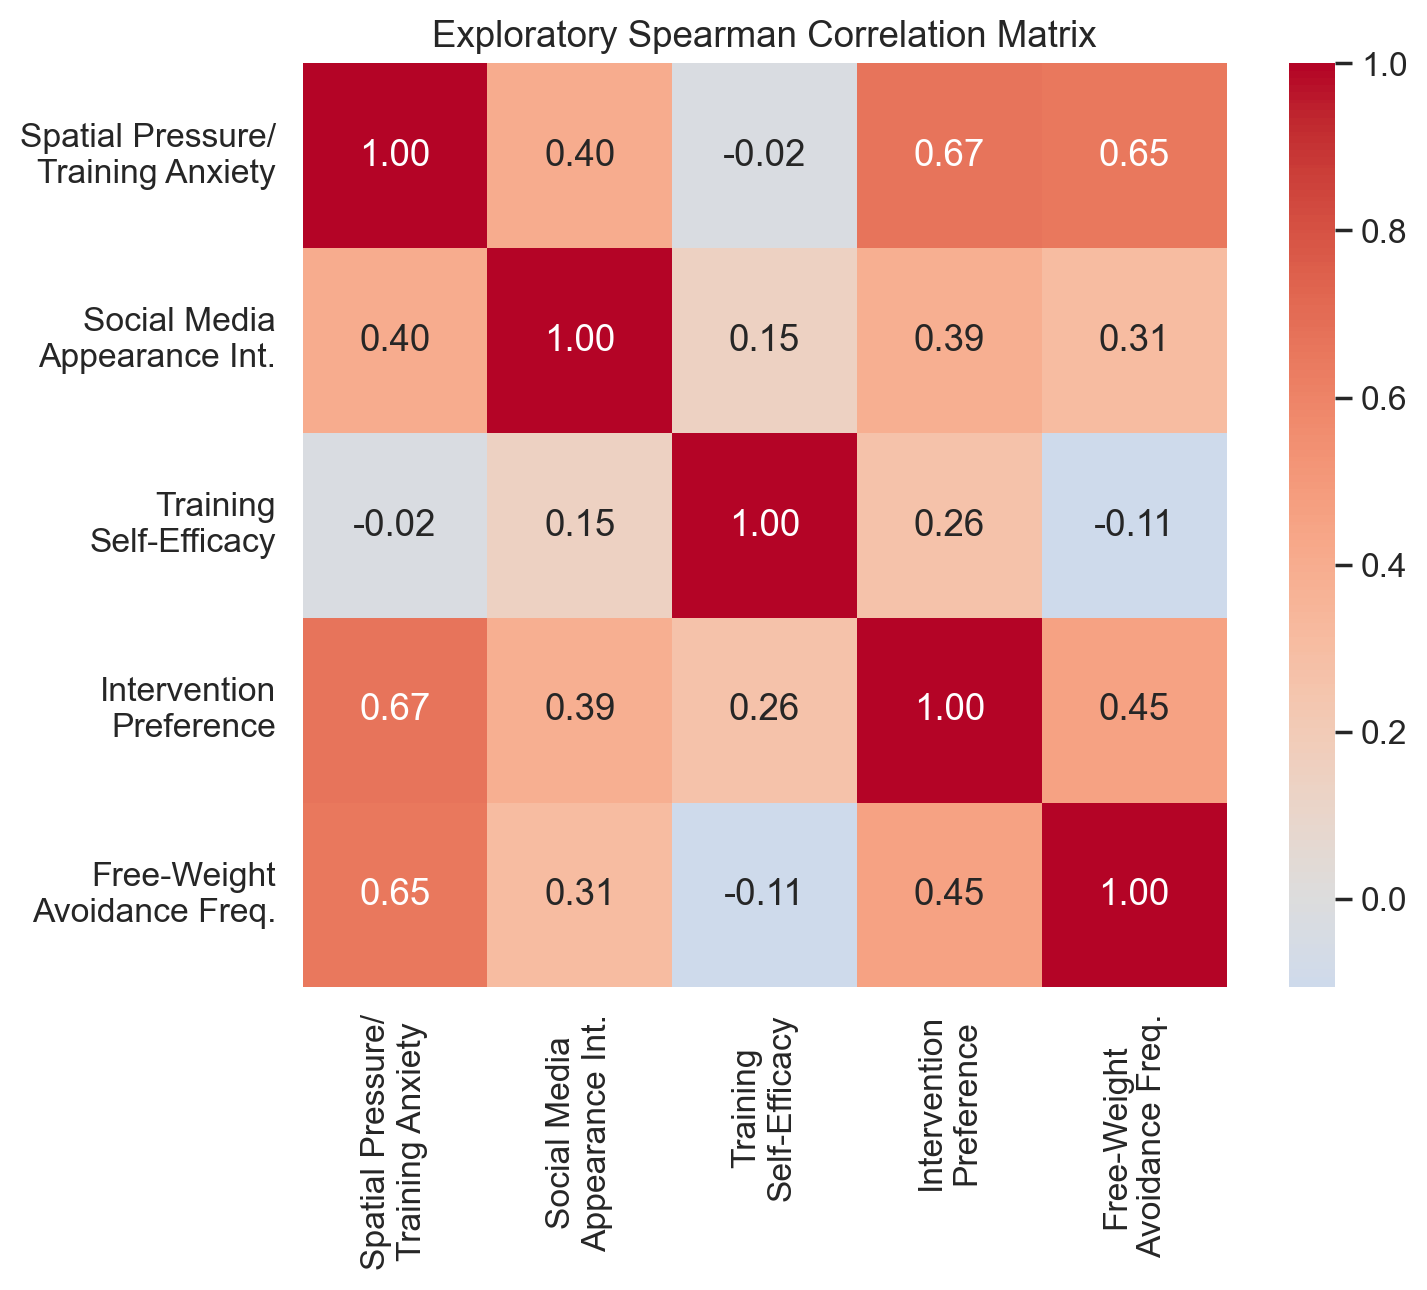
\includegraphics[width=0.78\textwidth]{survey_spearman_correlations.png}
\caption{Exploratory Spearman Correlation Matrix}
\label{fig:spearman_matrix}
\end{figure}

The frequency of actively avoiding the free-weight area also supports this picture.
Five participants (15.63\%) reported never avoiding, 5 (15.63\%) rarely avoiding, 10 (31.25\%) sometimes avoiding, and 6 (18.75\%) often avoiding.
In the aggregate export table, the ``always'' option was blank; however, since the valid sample for this item was 32 and the other options summed to 26 participants, ``always'' could be inferred as 6 participants (18.75\%).
In other words, at least 22 participants (68.75\%) sometimes or more frequently actively avoided the free-weight area.

Group comparisons also revealed differences between participants who actually entered the free-weight area and those who did not.
Only 5 participants most frequently used the free-weight area, so these results should be interpreted only exploratorily; however, this group's mean spatial pressure/training anxiety score was lower than that of non-regular users (2.60 vs.\ 3.92, Mann--Whitney $U = 16.00$, $p = .008$), and their avoidance frequency was also lower (1.40 vs.\ 3.41, $U = 10.00$, $p = .002$).
Participants with systematic strength training experience (currently or previously engaging in regular strength training, $n = 8$) also had lower avoidance frequency than those without systematic experience (1.88 vs.\ 3.50, $U = 28.00$, $p = .003$).
These differences cannot demonstrate that training experience directly reduces avoidance, but they suggest that familiarity with equipment and training procedures may co-occur with lower spatial pressure and avoidance tendencies.

Among the reasons for avoidance, the most frequently reported were ``too many men'' and ``do not know how to use equipment,'' both selected by 19 participants (59.38\%); followed by ``do not know where to start'' (16 participants, 50.00\%), ``no companion'' (11 participants, 34.38\%), ``fear of making form errors'' (9 participants, 28.13\%), and ``layout/atmosphere is too intimidating'' (8 participants, 25.00\%).
Notably, ``do not want to build visible muscle'' was selected by 0 participants (0.00\%).
Together with the social media items discussed below, this indicates that avoidance in this sample was not primarily driven by fear of becoming too muscular, but rather by a combination of spatial belonging, equipment knowledge, and evaluation pressure as a beginner.

\begin{figure}[H]
\centering
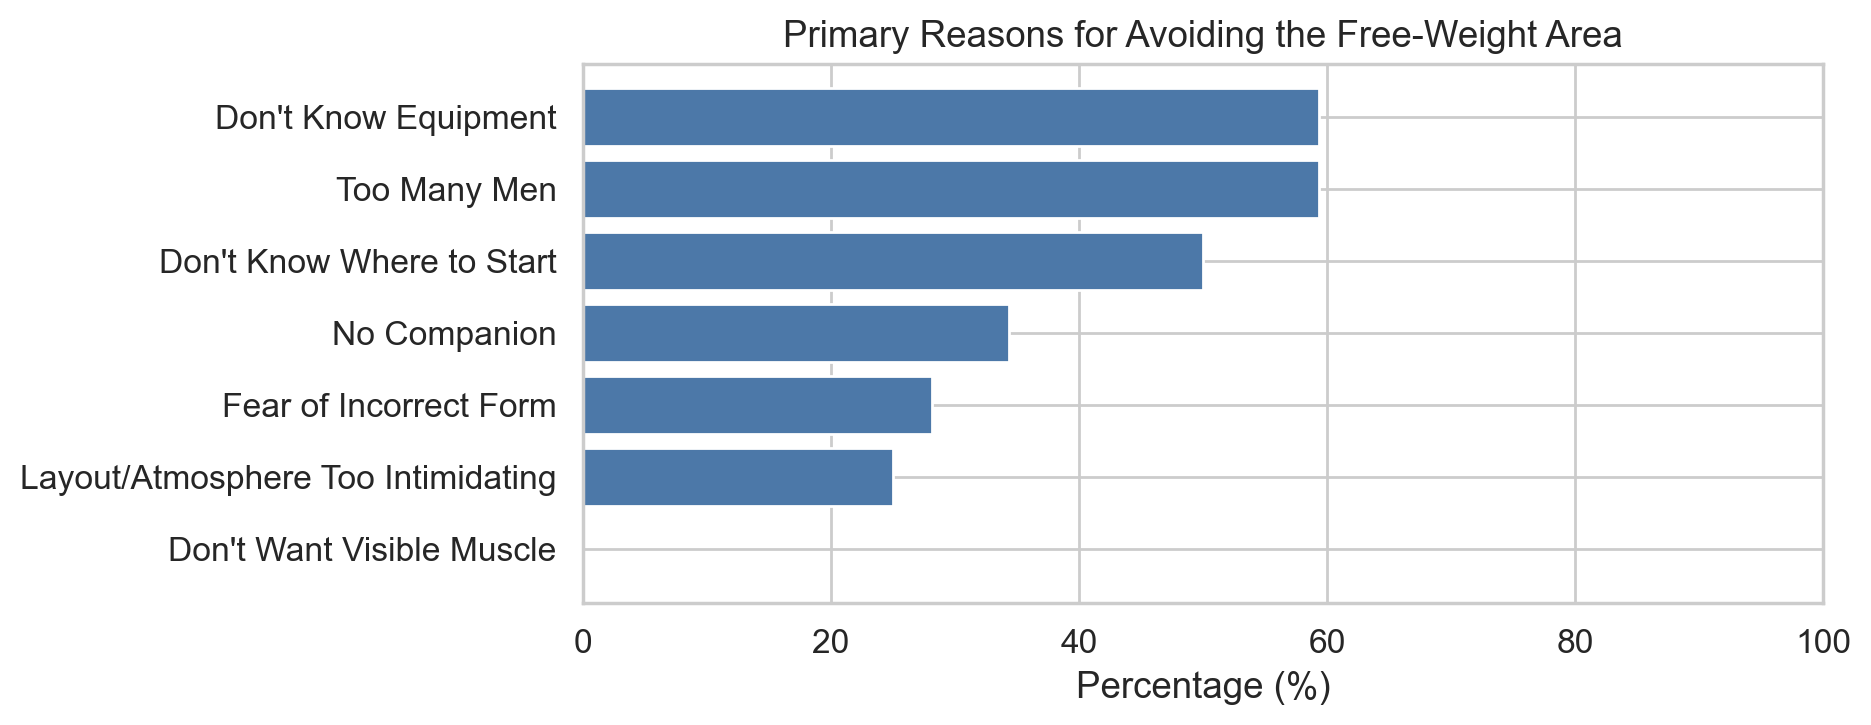
\includegraphics[width=0.85\textwidth]{avoidance_reasons.png}
\caption{Primary Reasons for Avoiding the Free-Weight Area (only options with explicit frequencies in the aggregate export table are shown)}
\label{fig:avoidance_reasons}
\end{figure}

\subsection{Social Media and Body Ideals}

Social media use was highly prevalent in the sample.
Xiaohongshu (RED) was the most frequently used platform (30 participants, 93.75\%), followed by Bilibili (22 participants, 68.75\%), Weibo (9 participants, 28.13\%), and Douyin/TikTok (8 participants, 25.00\%).
However, participants generally did not spend much time daily browsing body, fitness, fat loss, appearance, or outfit-related content: 14 participants (43.75\%) spent less than 15 minutes, 16 (50.00\%) spent 15--30 minutes, 2 (6.25\%) spent 31--60 minutes, and none selected more than 1 hour.

The social media appearance internalization construct comprised Items 21--23, with an individual-level mean of 2.66 ($SD = 0.93$) and acceptable internal consistency (Cronbach's $\alpha = .76$).
Among these items, ``Appearance-related content on social media influences what kind of exercise I choose'' had a mean of 3.40 and an upper score range of 59.38\%, indicating that appearance content does enter the exercise selection process.
However, ``I worry that strength training will make me look not slender enough or not conform to mainstream feminine aesthetics'' had a mean of only 1.85, with 81.25\% in the lower score range and only 15.63\% in the upper score range.
``I treat the female body standards popular on social media as my own goal'' had a mean of 2.73 and an upper score range of 31.25\%.
Thus, media influence in this study functioned more as a limited background factor in exercise selection rather than as a strong, unidirectional feminine aesthetic pressure.
Correlation analysis also supports this cautious interpretation: the correlation between social media appearance internalization and free-weight area avoidance frequency was positive but did not reach conventional significance ($\rho = .31$, $p = .084$), which was weaker than the relationship between spatial pressure/training anxiety and avoidance frequency.

\begin{table}[H]
\centering
\small
\caption{Social Media Appearance-Related Item Summary}
\label{tab:media_items_actual}
\begin{tabularx}{\textwidth}{lXccc}
\toprule
Item & Brief Description & Mean & Lower Score Range & Upper Score Range \\
\midrule
Q21 & Appearance content influences exercise choice & 3.40 & 21.88\% & 59.38\% \\
Q22 & Worry that strength training will not look slender or conform to feminine aesthetics & 1.85 & 81.25\% & 15.63\% \\
Q23 & Internalize popular social media female body standards & 2.73 & 43.75\% & 31.25\% \\
\bottomrule
\end{tabularx}
\end{table}

\begin{figure}[H]
\centering
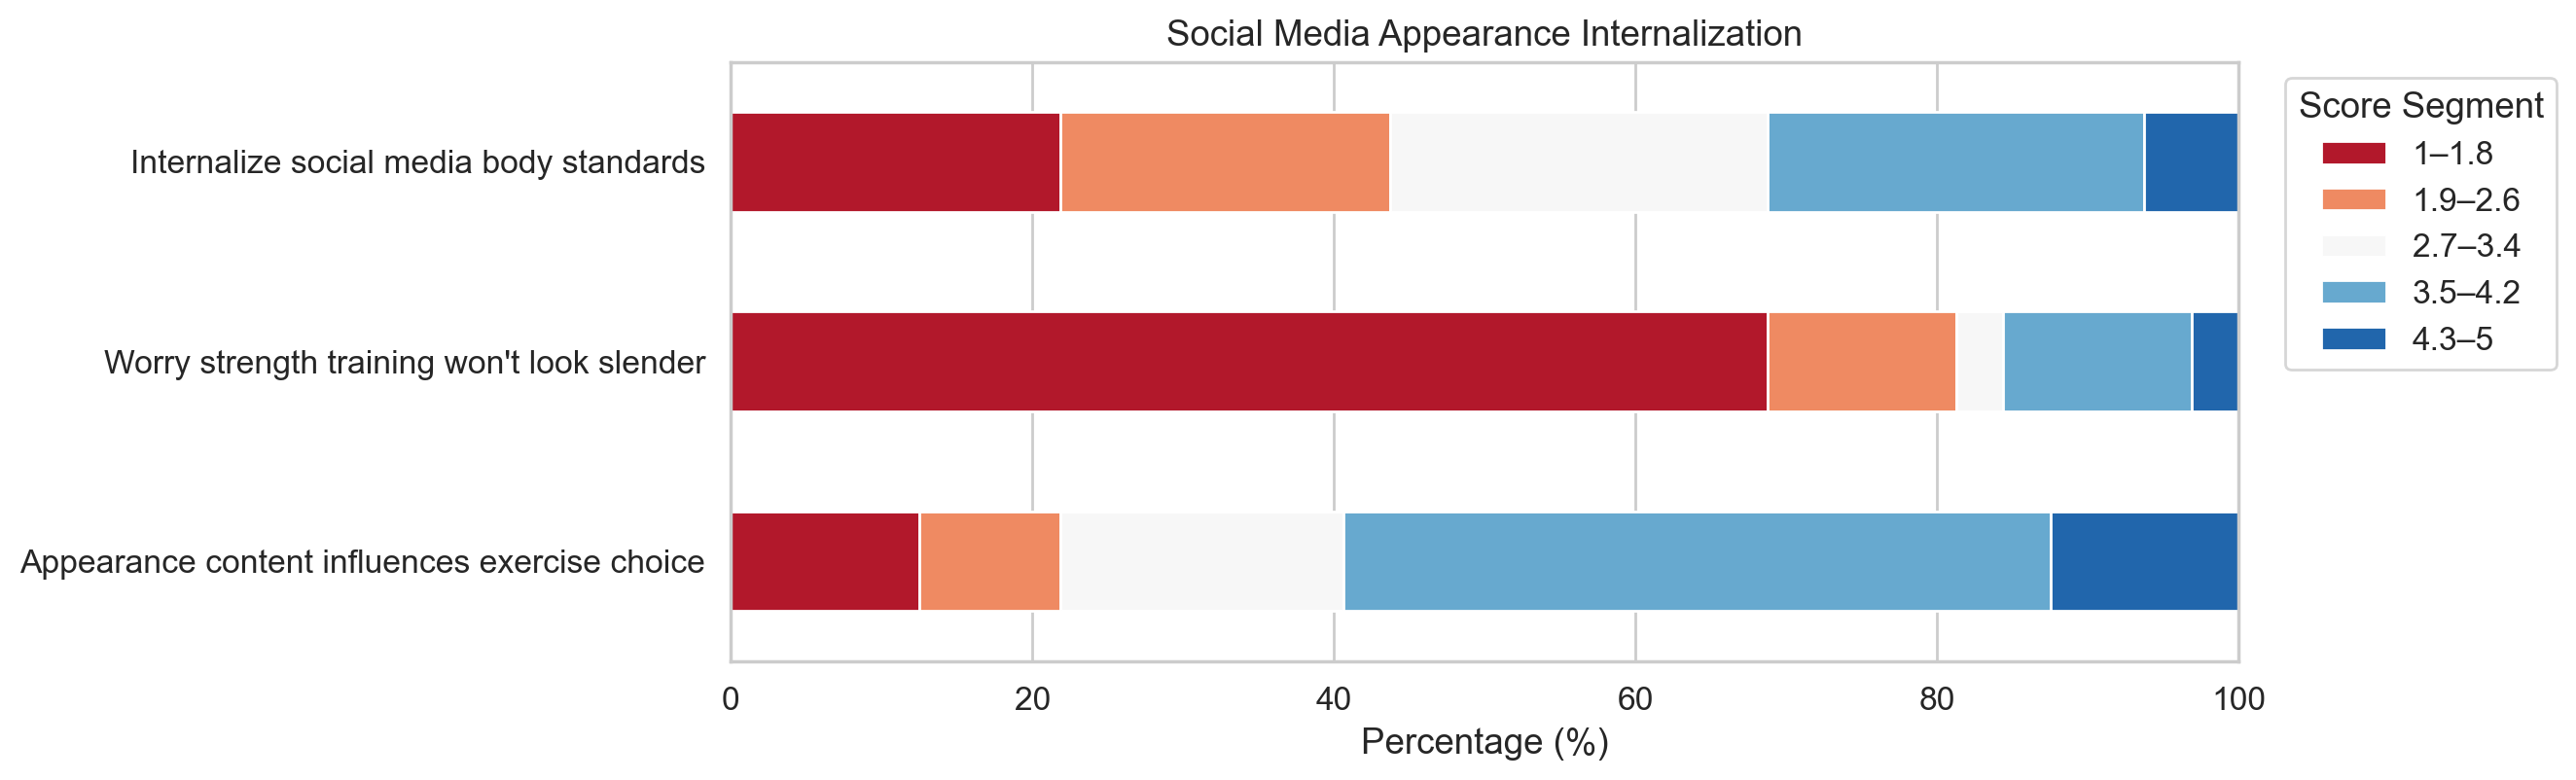
\includegraphics[width=0.85\textwidth]{slider_media_internalization.png}
\caption{Social Media Appearance-Related Slider Distribution}
\label{fig:media_distribution}
\end{figure}

\subsection{Self-Efficacy and Intervention Preferences}

Item 24 showed that participants' self-efficacy for achieving their training goals was at a moderate-to-upper level ($M = 3.49$, upper score range 50.00\%).
This suggests that many participants did not completely dismiss their ability to participate in gym training, but this confidence was insufficient to overcome the spatial and beginner barriers associated with the free-weight area.
Corroborating this interpretation, training self-efficacy showed virtually no association with free-weight area avoidance frequency ($\rho = -.11$, $p = .562$), indicating that general confidence in achieving training goals did not directly translate into willingness to enter the free-weight area.

The intervention preference index had the highest mean among all item sets, with an individual-level mean of 3.98 ($SD = 0.54$).
Because the three items measured three distinct interventions---media stereotype reduction, semi-private space, and beginner-friendly women's strength training workshops---this index was not interpreted as a strict psychological scale but rather as a descriptive indicator of overall support.
Among these items, ``If the university offered a beginner-friendly women's strength training workshop, I would be more willing to try strength training'' had a mean of 4.50 and an upper score range of 96.88\%.
``If semi-private partitioning or visual screening were added to the free-weight area, I would be more willing to use it'' had a mean of 4.04 and an upper score range of 81.25\%.
``If stereotypes about women's strength training on social media decreased, I would be more willing to participate in strength training'' had a mean of 3.39 and an upper score range of 50.00\%.
This ordering indicates that the most desired support was first university-based introductory guidance and spatial adjustments, followed by broader media stereotype improvement.
Notably, the intervention preference index was moderately positively correlated with free-weight area avoidance frequency ($\rho = .45$, $p = .009$), suggesting that participants who avoided the free-weight area more frequently were also more inclined to support these intervention measures---the strongest demand for change came from those most affected by the barriers.

\begin{figure}[H]
\centering
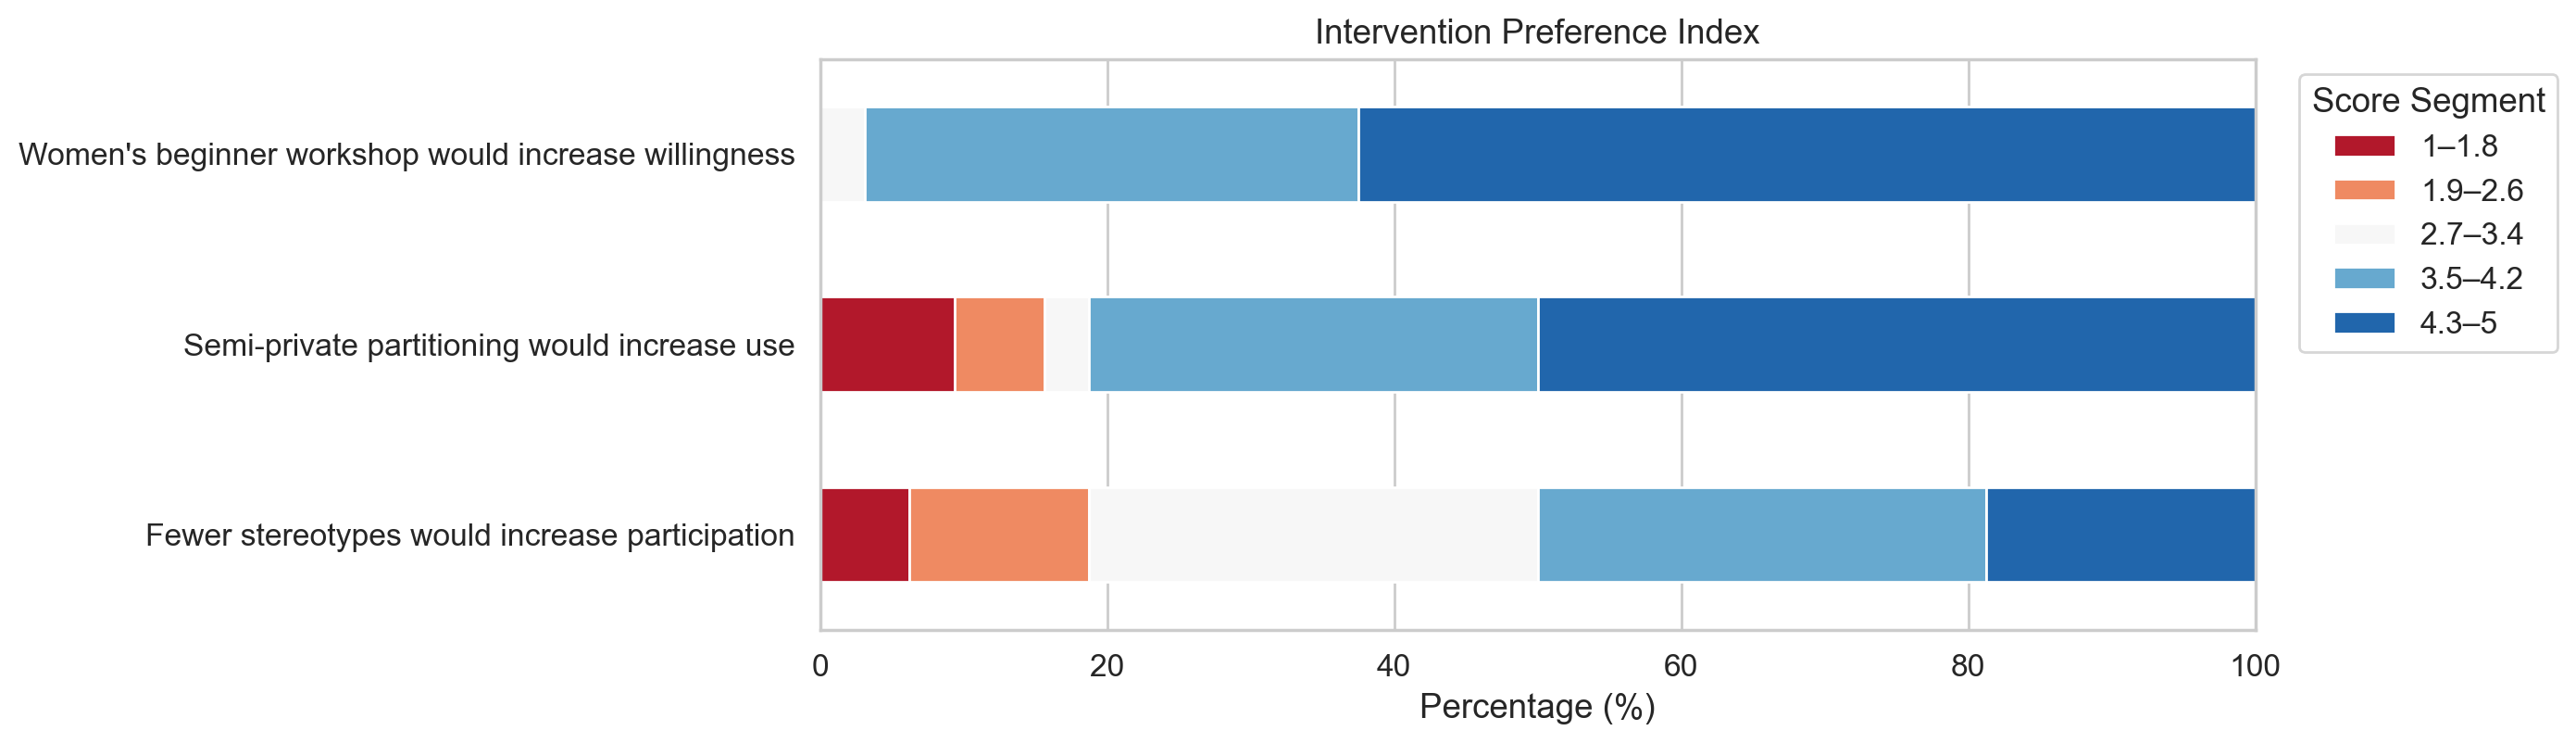
\includegraphics[width=0.85\textwidth]{slider_intervention_acceptance.png}
\caption{Intervention Preference Slider Distribution}
\label{fig:intervention_distribution}
\end{figure}

\subsection{Qualitative Themes}

The interview material yielded five themes directly related to the questionnaire results.
First, the strength training area was experienced as a space of heightened visibility.
P1 explained the difference between the cardio area and the strength area in terms of bodily orientation and mirrors: during cardio, one has one's ``back to others,'' while the strength area ``has mirrors,'' making it easier to see others and to become aware of being seen oneself.
P3 also mentioned that during strength training, ``there is a large mirror right in front, and it is easy to notice surroundings in peripheral vision,'' occasionally feeling that someone was looking at her.

Second, beginner barriers and fear of incorrect form were central obstacles.
P3 said that part of the reason she avoided the strength area was that she ``did not know how to do anything,'' worrying about not knowing how to use the equipment and having non-standard form, which might lead others to think she was ``really bad at this.''
P2 offered a similar explanation from a more measured perspective: many female students ``do not really understand strength training methods'' or how to use the tools, so when it is crowded, they worry about having non-standard form and delaying others' use of equipment.
This is consistent with the high frequency of selecting ``do not know how to use equipment'' and ``do not know where to start'' in the questionnaire.

Third, the male-dominated atmosphere created a sense of distance, but the interviewees did not interpret it simply as hostility from individual men.
P2 considered the gym to be well-equipped and that people were generally respectful, but also noted that the space felt crowded when busy, and the gym ``mostly looks like it was designed in a masculine style,'' with most lifters being male; consequently, female students might feel their experience and weight levels differed from others, creating embarrassment.
P3 similarly emphasized that the male lifters were well-trained with considerable muscle mass---this was not itself a target of criticism, but it could create a sense of intimidation for beginners.

Fourth, avoidance often took the form of strategic negotiation rather than complete withdrawal from exercise.
P1 would switch to cardio, find a roommate to accompany her, or go during less crowded times before 9 a.m.
P3 would choose not to wear glasses and go with a friend, relying on ``blocking out the surroundings'' to calm herself down.
In the questionnaire, the most common coping strategies were also going during off-peak timing (46.88\%), staying only in the cardio/fixed machine area (37.50\%), and giving up on strength training they had originally planned or leaving the gym (both 31.25\%).

Fifth, social media appearance influence existed, but the three interviewees each had different relationships with media content, and none translated appearance pressure into direct avoidance of strength training.
P1 frequently encountered fitness videos but reported ``not really seeing'' negative appearance-related evaluations; when she saw fit bodies, she thought ``that is great'' and ``did not really care what people said in the comments''---her engagement with social media fitness content was more appreciative than anxious.
P2 simultaneously encountered both positive and negative viewpoints but judged that ``the positive views are a bit more'' and believed that ``mainstream aesthetics are quite diverse nowadays''; regarding the claim that ``getting too muscular does not look good,'' although she ``felt uncomfortable,'' she resolved the conflict by redefining strength training---``fitness is not necessarily about getting bulky, but about making your muscles and posture better'' and ``as long as body fat percentage goes down, it is fine.''
P3 most directly rejected appearance pressure, ``completely disagreeing'' that strength training would deviate from mainstream aesthetics and ``sometimes even arguing back''; however, she mentioned that social media content about ``bad people and incidents'' at gyms could influence her overall impression of the gym, suggesting that social media influence may not operate through the appearance anxiety pathway but rather indirectly reduce willingness to enter by disseminating negative gym culture.
These three differentiated response patterns corroborate the asymmetric pattern found in the questionnaire---Q21 (appearance content influences exercise choice) had an upper score range of 59.38\%, but Q22 (fear of not looking slender enough from strength training) had a lower score range of 81.25\%: appearance content does enter participants' informational environment, but its role is more akin to a limited background influence rather than a mechanism directly driving avoidance.

\begin{table}[H]
\centering
\small
\caption{Integration of Interview Themes and Quantitative Results}
\label{tab:qual_themes_actual}
\begin{tabularx}{\textwidth}{lX}
\toprule
Theme & Relationship to Questionnaire Results \\
\midrule
Spatial visibility and mirror gaze & Explains Q12 upper score range of 53.13\% and interview accounts that the strength area produces a greater sense of being seen compared to the cardio area \\
Beginner barriers and fear of incorrect form & Corresponds to ``do not know how to use equipment'' 59.38\%, ``do not know where to start'' 50.00\%, and Q13 upper score range of 65.63\% \\
Male-dominated atmosphere and sense of distance & Corresponds to ``too many men'' 59.38\%, Q11 upper score range of 81.25\%, and Q14 upper score range of 62.50\% \\
Strategic negotiation rather than complete withdrawal & Corresponds to off-peak timing, switching to cardio/fixed machine area, and giving up planned strength training as coping strategies \\
Limited and diverse appearance influence & Corresponds to Q21 showing influence but Q22 scoring low, indicating media influence exists but is not a primary avoidance mechanism \\
Beginner-friendly/women-friendly intervention needs & Corresponds to beginner-friendly women's strength training workshop upper score range of 96.88\% and semi-private partitioning upper score range of 81.25\% \\
\bottomrule
\end{tabularx}
\end{table}

\section{Discussion}

\subsection{Space Matters More Than Abstract Disinterest}

The clearest finding of this study is that the female college students in the sample were not universally inactive, nor did they completely reject the gym; rather, they exhibited a pronounced threshold for entry specifically into the free-weight area.
Although 78.13\% of participants had used the campus gym and 46.88\% exercised 2--3 times per week, only 15.63\% most frequently used the free-weight area.
This discrepancy suggests that the issue should not be interpreted as ``women lack exercise interest,'' but rather as uneven participation resulting from spatial differentiation within the campus gym.

The mean score for spatial pressure/training anxiety reached 3.72, with discomfort when many men were present, pressure from crowded conditions, fear of incorrect form, and perceptions of male dominance all at moderate-to-high levels.
After supplementing the participant-level data, spatial pressure/training anxiety showed a strong positive correlation with the frequency of actively avoiding the free-weight area ($\rho = .65$), and regular users of the free-weight area also had notably lower spatial pressure scores than non-regular users.
Although this bivariate relationship cannot demonstrate causal direction, it reinforces the core explanation of this paper: avoidance is not an isolated attitude but co-occurs with specific spatial pressures.
This result resonates with \textcite{turnock2021gyms}'s finding that women in mixed-gender gyms feel tolerated rather than genuinely welcomed, and aligns with \textcite{rendall2024gym}'s identification of gym intimidation as an exercise barrier for female college students.
From the spatial theory perspective of \textcite{lefebvre1991production}, the free-weight area is not a neutral equipment zone; rather, it is produced---through mirrors, open visibility, bodily display, weight disparities, and gender ratios---as a social space with an entry threshold.

The interviews further revealed that this threshold does not arise solely from hostility on the part of individual men.
On one hand, interviewees acknowledged that most people were ``just doing their own workout''; on the other hand, they still felt overly visible due to mirrors, peripheral vision, equipment occupation, and unfamiliarity with exercises.
This aligns with the self-surveillance mechanism emphasized by objectification theory: even in the absence of explicit external evaluation, women may preemptively position themselves as being watched in visible spaces \parencite{fredrickson1997objectification,clark2018gaze}.
Thus, avoiding the free-weight area is better understood as a form of anticipatory management of visibility and the possibility of error, rather than simple timidity.
Notably, training self-efficacy showed virtually no correlation with avoidance frequency ($\rho = -.11$, $p = .562$), despite a moderate self-efficacy mean ($M = 3.49$); this suggests that the barrier lies not in participants' general confidence about achieving training goals but in the specific spatial and beginner-entry conditions of the free-weight area---further supporting the interpretation that avoidance is situationally driven rather than attributable to individual dispositions.

\subsection{Beginner Access as the Primary Barrier, With Indirect Media Effects}

The initial research framework hypothesized that social media appearance internalization might significantly drive resistance training avoidance, particularly through the concern that strength training would cause the body to deviate from the slender feminine ideal.
The actual data did not fully support this.
Although 59.38\% of participants agreed in Q21 that appearance content influenced their exercise choice, the mean for Q22 (``worry that strength training will not look slender enough'') was only 1.85, with 81.25\% in the lower score range.
Among avoidance reasons, ``do not want to build visible muscle'' also registered at 0\%.
The individual-level correlation similarly showed only a weak positive trend between social media appearance internalization and avoidance frequency ($\rho = .31$, $p = .084$), which was less robust than the spatial pressure variables.

This does not mean that social media is unimportant; rather, it indicates that its role in this sample was more indirect and complex.
Q21's mean reached 3.40 with an upper score range of 59.38\%, indicating that appearance content does influence the exercise selection process, but Q22's low scores suggest that this influence operates more at the goal level (e.g., making fat loss the most common exercise goal) without directly translating into a strong fear of muscular outcomes from strength training.
Both P2 and P3 in the interviews mentioned encountering related debates but did not agree with the claim that ``women who do strength training look bad.''
This is consistent with changes revealed by recent research on fitspiration and the fit-ideal: contemporary female body ideals are not exclusively about thinness but simultaneously incorporate elements of health, toning, strength, and displayability \parencite{tiggemann2015fitspiration,donovan2020fitideal}.

By contrast, the questionnaire and interviews more consistently pointed to the problem of ``how beginners enter.''
``Do not know how to use equipment'' and ``too many men'' were equally the most frequent avoidance reasons, and ``do not know where to start'' also reached 50.00\%.
Participants with systematic strength training experience had lower avoidance frequency than those without systematic experience; although limited by sample size, this result is consistent with the interview narrative that ``having learned/having someone teach'' can reduce uncertainty.
P2 began trying strength training after learning through a course, while P3, not knowing the equipment and movements, primarily performed bodyweight exercises in her dormitory.
This suggests that if the university only provides gym equipment without offering entry paths that beginners can understand, practice, and make mistakes in, formal resource accessibility will not automatically translate into actual participation.

\subsection{Strategic Negotiation Rather Than Passive Withdrawal}

This study also suggests that participants should not be portrayed as passive subjects entirely suppressed by spatial and appearance norms.
Many avoidance behaviors were actually strategic: going during off-peak hours, going when fewer people were present, finding a friend to go with, switching to the cardio or fixed machine area, and observing the environment before deciding whether to continue.
These practices show that participants were not uninterested in exercise but were seeking relatively controllable ways to enter a space where they did not feel entirely at ease.

This ``negotiated participation'' echoes \textcite{xiong2021fanshen}'s discussion of Chinese women's fitness narratives: women's fitness cannot be reduced to a singular narrative of ``being disciplined'' or ``being empowered,'' but involves continuous negotiation among body image, health management, social relationships, and self-identity.
In this study, women's participation in fitness could be organized by appearance norms, but it could also become a practice for enhancing physical capability, building self-care, and asserting spatial presence.
Specifically, P2 understood strength training as health and posture improvement, and P3, despite being nervous, still said she wanted to go to the gym in the future.
Therefore, resistance training avoidance should not be understood as a fixed identity but as a behavioral state that is repeatedly adjusted under specific spatial conditions.

It is worth noting that RQ3 originally focused on the negotiation between ``health motivation'' and ``digital appearance norms,'' but the data from this sample more consistently pointed to a different kind of negotiation---participants were primarily not choosing between health and appearance but rather seeking strategic ways to participate in a space that made them feel overly visible and lacked entry paths.
This shift itself corroborates the earlier findings: in this sample, spatial visibility and beginner barriers constituted more prominent obstacles than appearance pressure, and the core target of ``negotiation'' was spatial conditions rather than appearance norms.

\subsection{Practical Implications}

In practical terms, the most direct recommendation is not simply to encourage female students to ``be braver,'' but to lower the entry costs for beginners in the free-weight area.
The most popular intervention in the questionnaire was the beginner-friendly women's strength training workshop, with an upper score range reaching 96.88\%.
The correlation between spatial pressure/training anxiety and the intervention preference index was also high ($\rho = .67$), indicating that the demand for supportive interventions primarily came from participants who already perceived the free-weight area as difficult to enter.
Such workshops should focus on basic movements, equipment usage, weight selection, training programming, and common errors, rather than merely promoting body sculpting.
If these workshops could be led by female coaches, student assistants, or trained peer mentors, they might further reduce beginner discomfort in male-dominated spaces.

Second, spatial design should reduce the pressure of ``being seen as soon as you enter.''
Support for semi-private partitioning or visual screening was high (upper score range 81.25\%), and the interviews explicitly mentioned partitions, small spaces, fewer large mirrors, and greater attention to cleanliness.
This does not necessarily require complete gender segregation of the gym; rather, it can be achieved by distributing lighter equipment, setting up beginner practice corners, improving the relationship between mirrors and traffic flow, and providing clear equipment instructional videos, thereby creating lower-risk practice areas for beginners.

Third, campus communication should shift from ``slimming/fat loss'' toward functional, body-diverse, and beginner-friendly narratives.
Although this sample did not strongly worry that strength training would make them not slender enough, fat loss/slimming remained the most common exercise goal.
If university communications continue to present exercise as an appearance management project, they may reinforce body comparison; a more appropriate approach would be to emphasize the benefits of strength training for physical fitness, posture, bone health, menstrual health, and daily functional capacity, while showcasing women at different training levels and body types.

\subsection{Theoretical Reflection}

The three-layer integrated theoretical framework proposed in the literature review---spatial production, body objectification, and behavioral outcomes---effectively organized the findings of this study overall, but the level of support for each layer was asymmetric.
The first layer (spatial production) received the strongest support: the strong correlation between spatial pressure/training anxiety and avoidance frequency ($\rho = .65$), together with the interview narratives about mirrors, visibility, and the male-dominated atmosphere, jointly corroborated that the free-weight area is produced---through social relations---as a space with an entry threshold.
The second layer (appearance internalization) played a weaker role than initially anticipated: the correlation between social media appearance internalization and avoidance did not reach significance, and ``fear of getting bulky'' was virtually absent as an avoidance reason; however, Q21's high scores suggested that appearance content still influenced exercise goal selection, albeit operating primarily at the goal level rather than directly driving avoidance behavior.
The third layer (behavioral outcomes) was further enriched by the data: participants' behavior manifested not merely as a binary choice between avoidance and participation but as strategic negotiation situated between the two, which is consistent with \textcite{xiong2021fanshen}'s observation of ``neither fully disciplined nor fully empowered'' in women's fitness narratives.
This asymmetry is itself a finding---it suggests that among female college students lacking systematic strength training experience, spatial visibility and beginner barriers may be more proximal and direct obstacles than appearance internalization.
The mixed-methods design strengthened this interpretation through triangulation: the quantitative correlation ($\rho = .65$) between spatial pressure and avoidance established the direction and strength of the association, while the interview narratives provided the contextual mechanism---mirrors, male numerical dominance, fear of incorrect form, and equipment unfamiliarity---explaining why spatial pressure translates into avoidance behavior.
Conversely, the non-significant correlation between social media appearance internalization and avoidance ($\rho = .31$, $p = .084$) was enriched by the qualitative finding that interviewees' relationships with media content were differentiated and often dismissive, lending depth to what would otherwise be a merely negative statistical result.

\subsection{Limitations}

The greatest limitation of this study is the small sample size and single-campus context: the core questionnaire sample consisted of only 32 participants, and interviews involved only 3 individuals.
After supplementing the participant-level response matrix, this paper was able to calculate internal consistency, individual-level construct scores, Spearman correlations, and exploratory group comparisons; however, these results remain susceptible to the influence of outliers, group imbalance, and multiple comparisons.
Therefore, this paper does not conduct regression, mediation, or predictive modeling, nor does it interpret $p$ values as strong evidence.

Second, in some multiple-choice items, a minority of options were blank in the aggregate export table; this paper only reports options with explicit frequencies or those inferable from the valid sample size in the descriptive frequencies, and retains missing markers in the analysis script.
Third, the scale items were context-specific self-developed or adapted short items; although they drew on the theoretical dimensions of SEAM and SATAQ-4, they have not undergone full psychometric validation.
In particular, the three intervention preference items measured different policy/spatial proposals and should not be over-interpreted as a single psychological scale.
Fourth, this study used cross-sectional self-report data, which cannot determine whether spatial pressure causes avoidance or whether students who already avoid the free-weight area are more likely to evaluate that space as intimidating in their imagination.

Future research should preserve participant-level raw response data, expand the sample to multiple universities, and employ fully validated scales or formally validated Chinese short-form instruments.
If conditions permit, researchers could compare free-weight area usage before and after participation in a beginner-friendly women's strength training workshop, thereby more directly evaluating whether workshops and spatial interventions can reduce resistance training avoidance.

\section{Conclusion}

Based on questionnaire data from 32 female college students and 3 semi-structured interviews, this study examined the relationships among gym spatial environment, body image, and resistance training avoidance in a Chinese/Asian campus context.
The results showed that participants were not lacking in exercise interest: the majority had used the campus gym and maintained a regular exercise frequency.
However, utilization of the free-weight area was notably low, with 68.75\% of the sample actively avoiding the free-weight area at least ``sometimes.''
Participant-level data further revealed a relatively strong positive association between spatial pressure/training anxiety and free-weight area avoidance frequency, whereas the relationship between social media appearance internalization and avoidance was weaker.
The most prominent barriers were not concern about building visible muscle, but rather the male-dominated environment, unfamiliarity with equipment, not knowing where to begin, fear of incorrect form, and the discomfort caused by open, visible spaces.

Social media appearance content may influence exercise goal selection for some individuals ($\rho = .31$, $p = .084$), but the present sample did not exhibit a strong anxiety that ``strength training will undermine a slender feminine image.''
Interviews also revealed that respondents frequently held reserved or even dismissive attitudes toward relevant stereotypes.
Therefore, the central conclusion of this paper is: in the Chinese/Asian campus context of the present sample, resistance training avoidance among female college students in campus gyms is more primarily a spatial and beginner barrier issue rather than solely an appearance internalization issue.

Regarding RQ3, this study originally hypothesized that participants would negotiate between health motivation and digital appearance norms, but the actual data more consistently pointed to a different form of negotiation: participants primarily sought strategic ways to participate within a space where they felt overly visible and lacked entry pathways, rather than making trade-offs between health and appearance. This shift is itself consistent with the preceding findings---in the present sample, spatial visibility and beginner barrier constituted more salient obstacles than appearance pressure, and the core object of ``negotiation'' was spatial conditions rather than appearance norms.

In practice, universities should prioritize beginner-friendly women's strength training workshops, equipment instruction, companion support, and semi-private/beginner-friendly spatial modifications.
These measures can transform ``having a gym'' into genuine accessibility characterized by ``daring to enter, knowing how to use equipment, and being able to sustain practice.''

Theoretically, this study demonstrates the value of analyzing spatial production, body objectification, and behavioral choices within a single framework. When ``the space does not belong to me'' and ``my body must not deviate from ideal femininity'' co-occur, spatial visibility and beginner barrier constitute more prominent obstacles than appearance internalization in the present sample. This suggests that future research should not understand women's resistance training avoidance solely from the single perspective of body image or exercise participation, but should attend to how gym spaces are experienced as social fields with entry barriers.

Given the limited sample size of this study and the fact that all individual-level statistics are exploratory bivariate analyses, the conclusions should not be extrapolated as causal laws; however, the findings clearly suggest that gender equity in campus gyms depends not only on equipment availability, but also on how spaces are experienced, who is able to make mistakes and learn within them, and whether female beginners can be seen as legitimate users.


% ── 生成式 AI 使用说明 ──
\section*{Use of Generative AI}
\addcontentsline{toc}{section}{Use of Generative AI}
Generative AI tools were used as auxiliary support for coding assistance, data-cleaning workflow design, drafting support, language polishing, and preliminary consistency checks. All quantitative interpretations, qualitative themes, literature use, and final arguments were reviewed and revised by the authors against the available survey export, interview transcripts, assignment brief, proposal, and cited sources.

% ── 参考文献 ──
\printbibliography[heading=bibintoc, title={References}]

\end{document}
